\section{Designing and Creating the generator artifact} \label{sec_generator_artifact}

In the previous chapters, we discussed the importance of software stability and
evolvability in order to cope with the continuously changing business and technological
requirements. Although considered from a much broader perspective, the Greek philosopher
\emph{Heraclitus} described this state of constant \emph{flux} with his famous statement
\emph{Pantha Rhei}. His statement was the main inspiration for the name of the generator
artifact.

The following sections discuss the design, implementations and functionality of the Pantha
Rhei, the generator artifact. The artifact is created in fulfillment of this research.
Whereas the name of the artifact was inspired by Heraclitus, the functional idea behind
the artifact was inspired by the theory behind \gls{ns} and by the Prime Radiant
application of the company NSX
\footnote{\url{https://normalizedsystems.org/prime-radiant/}}. The concept of code
generation in order to achieve stable and evolvable software is one of the important aspects
of \gls{ns}.

For the interested readers of this thesis, it is rather simple to install the Pantha Rhei
application by following the instruction in the appendix
\fullref{appendix_installation_instructions}.

\section{Expanders}

The Exander Framework allows for the miscellaneous execution of expanders of any type. The
Expander Framework is independent of any of the details of Expanders, fully adhering to
the principle of \gls{dip}. Conversely, an Expander is required to implement several
interfaces to ensure execution and dependency management are available during runtime. The
Expander Framework also consists of a set of default tasks, such as the execution of the
expansion tasks known as ExpanderHandlerInteractors
\citecode{koks_iexpanderhandlerinteractor_2023}, logging, bootstrapping dependencies, and
tasks to execute harvestings and injections. Except for the use of the
IExpanderInteractor, non of which are required.

Figure \ref{fig_expander_design} illustrates the dependencies between the domain layer of
the Expander Framework. The Clean Architecture Expander is considered an application layer
containing specific tasks bounded to a particular application or process. In this case,
the Expansion process.

\begin{figure}[H]
    \centering
    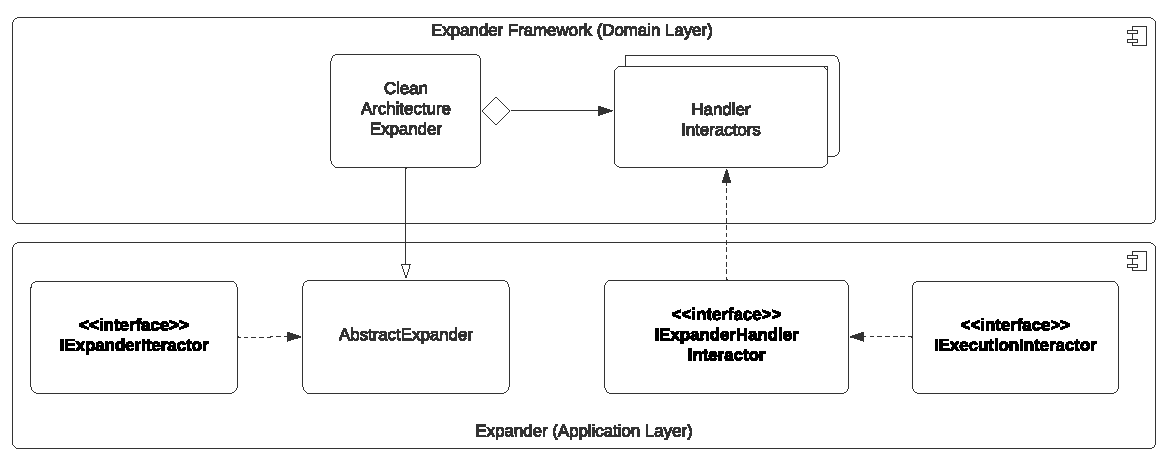
\includegraphics[width=1\textwidth]{figures/expander.pdf}
    \caption[The design of an Expander]{The design of an Expander}
    \label{fig_expander_design}
  \end{figure}
\input{chapters/artifacts/generator/pluginarchitecture}
\subsection{The executer object} \label{subsec_IExecutionInteractorObject}

A vital implementation that facilitates a high degree of cohesion, whilst maintaining
low coupling and adhering to the \gls{srp} principle is the use of the
\citecode{koks_iexecutioninteractor_2023} interface. The generation process is designed to
execute \enquote{tasks} in a predefined order. By using the
\code{koks_iexecutioninteractor_2023} it is possible to design each of the tasks as
separate classes, entirely complying, or enabling all of the \gls{solid} principles. The 

\begin{figure}[H]
    \centering
    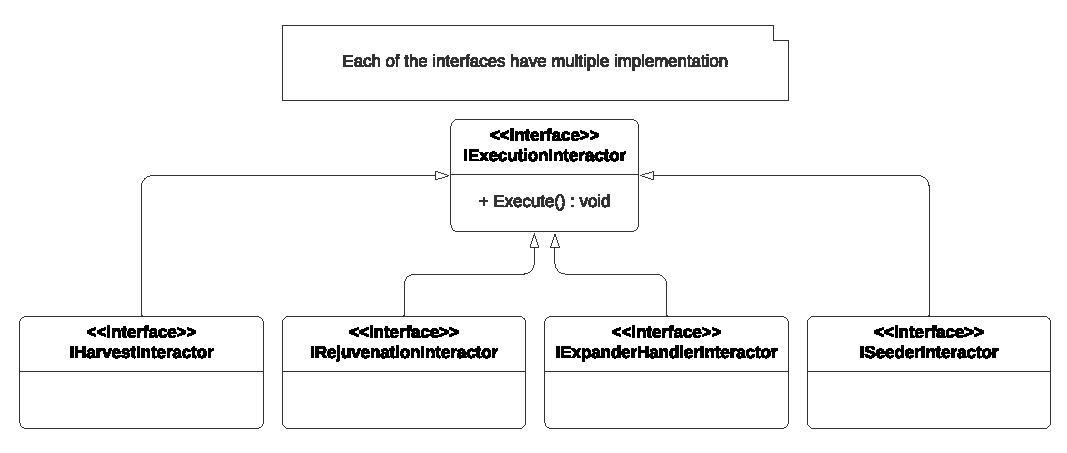
\includegraphics[width=1\textwidth]{figures/class_diagram_iexecutioninteractor.pdf}
    \caption[Plugin Archticture]{Both high cohesion and low coupling by using the \code{koks_iexecutioninteractor_2023}}
    \label{fig_iexecutioninteractor}
  \end{figure}


As depicted in listing \ref{list_CodeGeneratorInteractor}, this design leads to a cohesive
design where all tasks are gracefully executed from a single point in the application.
\lstinputlisting[
  caption={The \citetitle{koks_codegeneratorinteractor_2023}},
  label={list_CodeGeneratorInteractor} ] 
  {Snippets/CodeGeneratorInteractor.cs}
\chapter{The Entity Relationship Diagram of the Meta Mode} \label{appendix_metamodel_description}  

\section{The App entity}

The App entity represents the application and is regarded as the entry point for the
model. The App Entity and the subsequent entities contain all the information required to
perform the expandsion of a software system. 

\begin{table}[H]
    \small
    \begin{tabular}{ p{0.21\linewidth} p{0.21\linewidth} p{0.49\linewidth} }
        \hline
        \textbf{Name} & \textbf{DataType} & \textbf{Description} \\
        \hline
        Id & Guid & Unique identifier of the application \\
        Name & string & Name of the application \\
        FullName & string & Full name of the application \\
        Expanders & List of Expanders & The Expanders that will be used during the
        generation process. \\
        Entities & List of Entities & The Entities that are applicable for the Generated artifact. \\
        ConnectionStrings & List of ConnectionStrings & The ConnectionString to the
        database that is used by the Generator Artifact. \\
        \hline
    \end{tabular}
    \caption{The fields of the App entity}
    \label{table:app_entity}
\end{table}

\section{The Component entity}

The Component entity represents a software component that can be part of an application.
Based on this entity the Generator Artifact can make design time on where to place certain
elements  

\begin{table}[H]
\small
\begin{tabular}{ p{0.20\linewidth} p{0.20\linewidth} p{0.50\linewidth} }
\hline
\textbf{Name} & \textbf{DataType} & \textbf{Description} \\
\hline
Id & Guid & Unique identifier of the component \\
Name & string & Name of the component \\
Description & string & Description of the component \\
Packages & List of Package & The Packages that should be applied to the component. \\
Expander & Expander & Navigation property to the Expander entity. \\
\hline
\end{tabular}
\caption{The fields of the Component entity}
\label{table:component_entity}
\end{table}

\section{The ConnectionString entity}

The ConnectionString entity represents a ConnectionString used by an application to
connect to a database or other external system.

\begin{table}[H]
\small
\begin{tabular}{ p{0.20\linewidth} p{0.20\linewidth} p{0.50\linewidth} }
\hline
\textbf{Name} & \textbf{DataType} & \textbf{Description} \\
\hline
Id & Guid & Unique identifier of the ConnectionString \\
Name & string & Name of the ConnectionString \\
Definition & string & Definition of the ConnectionString \\
App & App & Navigation property to the App entity \\
\hline
\end{tabular}
\caption{The fields of the ConnectionString entity}
\label{table:connectionstring_entity}
\end{table}

\section{The Entity entity}

The Entity entity represents an entity in the application's data model. 

\begin{table}[H]
\small
\begin{tabular}{ p{0.20\linewidth} p{0.23\linewidth} p{0.47\linewidth} }
\hline
\textbf{Name} & \textbf{DataType} & \textbf{Description} \\
\hline
Id & Guid & Unique identifier of the entity \\
Name & string & Name of the entity \\
Callsite & string & The source code location where the entity is defined. In the case of a C\#
artifact, this is to determine the name of the namespace.\\
Type & string & Type of the entity \\
Modifier & string & Modifier of the entity (e.g. public, private) \\
Behavior & string & The behavior of the entity (e.g. abstract, virtual) \\
App & App & Navigation property to the App entity. \\
Fields & List of Fields & The Fields property represents a collection of the fields that
make up the entity. \\
ReferencedIn & List of Fields & Represents a navigation property to a Field that uses the
current entity as a return type. \\
Relations & List of Relationships & List of relationships involving this entity \\
IsForeignEntityOf & List of Relationships & List of relationships where this entity is the foreign entity \\
\hline
\end{tabular}
\caption{The fields of the Entity entity}
\label{table:entity_entity}
\end{table}

\section{The Expander entity}

The Expander entity represents an expander, which is responsible for generating code for
an application. The Generator Artifact attempts to execute all expanders that are related
to the selected App.

\begin{table}[H]
\small
\begin{tabular}{ p{0.20\linewidth} p{0.22\linewidth} p{0.48\linewidth} }
\hline
\textbf{Name} & \textbf{DataType} & \textbf{Description} \\
\hline
Id & Guid & Unique identifier of the expander \\
Name & string & Name of the expander \\
TemplateFolder & string & relative path to the templates that are used by the expander. \\
Order & int & The order in which the expander is executed \\
Apps & List of Apps & List of applications associated with the expander. \\
Components & List of Components & List of components associated with the expander \\
\hline
\end{tabular}
\caption{The fields of the Expander entity}
\label{table:expander_entity}
\end{table}

\section{The Field entity}

The Field entity represents a field or property of an entity in an application's data
model. Each field has a unique ID, name, and other properties such as its return type,
modifiers, and behavior. It can be associated with an entity and can have relationships
with other entities. The IsKey and IsIndex properties indicate whether the field is part
of the primary key or an index of the entity, respectively.

\begin{table}[H]
\small
\begin{tabular}{ p{0.23\linewidth} p{0.23\linewidth} p{0.45\linewidth} }
\hline
\textbf{Name} & \textbf{DataType} & \textbf{Description} \\
\hline
Id & Guid & Unique identifier of the field \\
Name & string & Name of the field \\
ReturnType & string & Return type of the field \\
IsCollection & bool & Whether the field is a collection or not \\
Modifier & string & Modifier of the field (e.g. public, private) \\
GetModifier & string & Modifier of the get accessor for the field \\
SetModifier & string & Modifier of the set accessor for the field \\
Behavior & string & The behavior of the field (e.g. abstract, virtual) \\
Order & int & The order of the field within its entity \\
Size & int? & The size of the field \\
Required & bool & Whether the field is required or not \\
Reference & Entity & The entity that this field refers to\\
Entity & Entity & A navigation property to the parent entity \\
IsKey & bool & Indicates whether the field is part of the primary key \\
IsIndex & bool & Indicates whether the field is part of an index \\
RelationshipKeys & List of Relationships & A List of entities that are defined as relations. \\
IsForeignEntityKeyOf & List of Relationships & List of relationships to the field that is the foreign key \\
\hline
\end{tabular}
\caption{The fields of the Field entity}
\label{table:field_entity}
\end{table}

\section{The Package entity}

The Package entity represents a software package that can be used by a component. This
could either be a Nuget package in the case of .NET projects, or for example npm packages
for web projects.

\begin{table}[H]
\small
\begin{tabular}{ p{0.20\linewidth} p{0.20\linewidth} p{0.50\linewidth} }
\hline
\textbf{Name} & \textbf{DataType} & \textbf{Description} \\
\hline
Id & Guid & Unique identifier of the package \\
Name & string & Name of the package \\
Version & string & Version of the package used \\
Component & Component & Component associated with the package \\
\hline
\end{tabular}
\caption{The fields of the Package entity}
\label{table:package_entity}
\end{table}

\section{The Relationship entity}

The Relationship entity represents a relationship between two entities in the App's data
model. The Relationship entity has proper cardinality support. Relationships are
bidirectional and can be navigated from either entity.

\begin{table}[H]
\small
\begin{tabular}{ p{0.24\linewidth} p{0.12\linewidth} p{0.55\linewidth} }
\hline
\textbf{Name} & \textbf{DataType} & \textbf{Description} \\
\hline
Id & Guid & Unique identifier of the relationship \\
Key & Field & The key field of the relationship \\
Entity & Entity & Navigation property to the parent Entity \\
Cardinality & string & The cardinality of the relationship \\
WithForeignEntityKey & Field & The foreign key field of the relationship, pointing to a
Field entity. \\
WithForeignEntity & Entity & The entity associated with the foreign key field \\
WithCardinality & string & The cardinality of the relationship with the foreign entity \\
Required & bool & indicates whether the relationship is required or not \\
\hline
\end{tabular}
\caption{The fields of the Relationship entity}
\label{table:relationship_entity}
\end{table}


